\documentclass[border=5pt]{standalone}
\usepackage{tikz}
\usetikzlibrary{calc, positioning}
\usepackage{amsmath}
\begin{document}
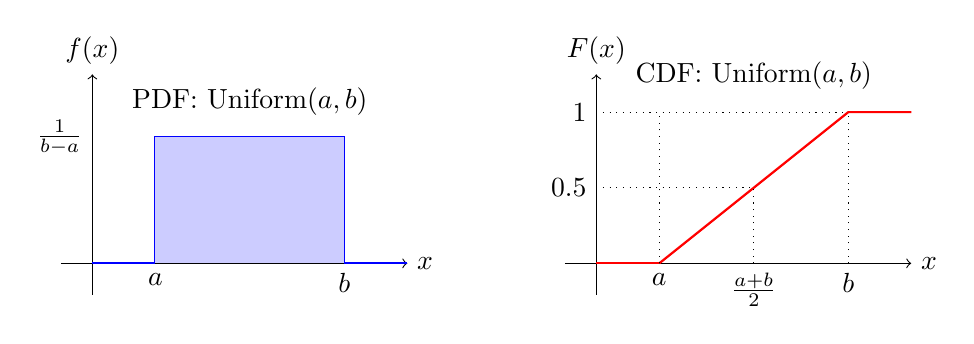
\begin{tikzpicture}[scale=0.8]
    % PDF subplot
    \begin{scope}[xshift=-4cm]
        % Axes
        \draw[->] (-0.5,0) -- (5,0) node[right] {$x$};
        \draw[->] (0,-0.5) -- (0,3) node[above] {$f(x)$};

        % PDF rectangle
        \draw[thick, blue] (1,0) -- (1,2) -- (4,2) -- (4,0);
        \draw[thick, blue] (0,0) -- (1,0);
        \draw[thick, blue] (4,0) -- (5,0);

        % Labels
        \node[below] at (1,0) {$a$};
        \node[below] at (4,0) {$b$};
        \node[left] at (0,2) {$\frac{1}{b-a}$};
        \node[above] at (2.5,2.2) {PDF: Uniform$(a,b)$};

        % Fill area
        \fill[blue!20] (1,0) rectangle (4,2);
    \end{scope}

    % CDF subplot
    \begin{scope}[xshift=4cm]
        % Axes
        \draw[->] (-0.5,0) -- (5,0) node[right] {$x$};
        \draw[->] (0,-0.5) -- (0,3) node[above] {$F(x)$};

        % CDF line
        \draw[thick, red] (0,0) -- (1,0);
        \draw[thick, red] (1,0) -- (4,2.4) -- (5,2.4);

        % Labels
        \node[below] at (1,0) {$a$};
        \node[below] at (4,0) {$b$};
        \node[left] at (0,2.4) {$1$};
        \node[left] at (0,1.2) {$0.5$};
        \node[above] at (2.5,2.6) {CDF: Uniform$(a,b)$};

        % Dotted lines for reference
        \draw[dotted] (1,0) -- (1,2.4);
        \draw[dotted] (4,0) -- (4,2.4);
        \draw[dotted] (0,2.4) -- (4,2.4);
        \draw[dotted] (0,1.2) -- (2.5,1.2);
        \draw[dotted] (2.5,0) -- (2.5,1.2);
        \node[below] at (2.5,0) {$\frac{a+b}{2}$};
    \end{scope}
\end{tikzpicture}
\end{document}
